\documentclass[a4paper, twocolumn]{article}

\usepackage{colortbl}
\usepackage{cancel}
\usepackage{diagbox}
\usepackage{siunitx}
\usepackage{multirow}
\usepackage{array}
\usepackage[table, xcdraw, dvipsnames]{xcolor}
\usepackage{times}
\usepackage{tikz}
\usepackage[top=0.75in, bottom=1in, inner=0.75in, outer=0.75in,
            headheight=45pt, headsep=2pt, footskip=5mm]{geometry}
\usepackage{graphicx}
\usepackage{anyfontsize}
\usepackage{fancyhdr}
\usepackage{indentfirst}
\usepackage{amsmath}
\usepackage[spanish, es-tabla]{babel}
\usepackage[utf8]{inputenc}
\usepackage[explicit]{titlesec}
\usepackage{etoolbox}
\usepackage{enumitem}
\usepackage[labelformat=simple,labelsep=none]{caption}
\usepackage{mathptmx}
\usepackage{lastpage}
\usepackage{booktabs}
\usepackage{amsfonts}
\usepackage[version=4]{mhchem}
\usepackage{float}
\usepackage{circuitikz}
\usepackage{subcaption}
\usepackage{changepage}
\usepackage{eso-pic}
% \usepackage{showframe}
\usepackage{minted}
\usepackage{pgfplots}
\pgfplotsset{compat=1.18}


\newcommand{\inicioCodigo}{
    \newpage
    \fancyfoot[C]{}
    \onecolumn
}

\newcommand{\finalCodigo}{
    \newpage
    \fancyfoot[C]{
        \begin{tikzpicture}[remember picture, overlay]
            \draw[gray!30, line width=0.4pt]
                (0cm, 1cm) -- (0cm, 25cm);
        \end{tikzpicture}
    }
    \twocolumn
}

\renewcommand{\theenumi}{\Roman{enumi}}
\definecolor{gold}{rgb}{1.0, 0.84, 0.0}
\newcommand{\resistencia}[4]{
    \begin{minipage}{2cm}
        \begin{center}
            \begin{tikzpicture}
                \draw(-0.4cm, -0.15cm) rectangle (0.4cm, 0.15cm);
                \fill[resistor] (-0.4cm, 0) -- (-0.5cm, 0);
                \draw (-0.4cm, 0) -- (-0.5cm, 0);
                \draw (0.4cm, 0) -- (0.5cm, 0);
                \fill[#1] (-0.35cm, -0.15cm) rectangle (-0.25cm, 0.15cm);
                \fill[#2] (-0.15cm, -0.15cm) rectangle (-0.05cm, 0.15cm);
                \fill[#3] (0.05cm, -0.15cm) rectangle (0.15cm, 0.15cm);
                \fill[#4] (0.25cm, -0.15cm) rectangle (0.35cm, 0.15cm);
            \end{tikzpicture}
        \end{center}
    \end{minipage}
}
\newcommand{\diodoSilicio}[1]{
    \begin{minipage}{2cm}
        \begin{center}
            \begin{circuitikz}[scale=0.5]
                \draw[line width=1pt] (-2,0) -- (-1,0);
                \draw[line width=1pt] (2,0) -- (1,0);

                \filldraw[fill=black!75, draw=black] (-1, -0.5) rectangle (1, 0.5);

                \fill[gray!60] (0.6, -0.5) rectangle (0.8, 0.5);

                \node at (0, -1) {\texttt{#1}};
            \end{circuitikz}
        \end{center}
    \end{minipage}
}
\newcommand{\diodoGermanio}[1]{
    \begin{minipage}{2cm} 
        \begin{center}
            \begin{circuitikz}[scale=0.5]
                \draw[line width=0.8pt] (-2.5,0) -- (-1.5,0);
                \draw[line width=0.8pt] (2.5,0) -- (1.5,0);

                \filldraw[fill=white, draw=black] (-1.5, -0.4) rectangle (1.5, 0.4);
                \fill[orange!80] (-1.5, -0.25) rectangle (1.5, 0.25);
                \fill[gray!95] (1.2, -0.4) rectangle (1.5, 0.4);
                \node at (0, -0.9) {\texttt{#1}};
            \end{circuitikz}
        \end{center}
    \end{minipage}
}
\newcommand{\inv}[1]{\frac{1}{#1}}
\newcommand{\recuadrar}[2]{
    \begin{center}
        \begin{tabular}{|m{#1}|}
            \toprule
            \multicolumn{1}{|c|}{\hspace{5pt}#2\hspace{5pt}} \\
            \bottomrule
        \end{tabular}
    \end{center}
}

\newcommand{\ecuacion}[1]{
    \begin{center}
        $#1$
    \end{center}
}

\newcommand{\longsection}[2]{%
    \section[#1]{\parbox{\columnwidth}{#1}}
}

\newcommand{\saltoPag}[0]{%
    \newpage\noindent\thispagestyle{fancy}%
    \begin{tikzpicture}[remember picture, overlay]
        \draw[line width=0.4pt, color=gray!50] (8.5cm, -0.4cm) -- (8.5cm, -24cm);
    \end{tikzpicture}%
    \ignorespaces{}
}

\newcommand{\midTitle}[2]{%
    \begin{center}
        \textcolor{#1}{\underline{#2}} 
    \end{center}
}

\captionsetup{
    format=hang,
    labelfont={bf},
    textfont=normalfont,
    labelsep=colon,
    justification=centering,
    singlelinecheck=true
}

\newcommand{\imagen}[3][]{
    \begin{center}
        \begin{tikzpicture}
            \node[inner sep=2pt] (image) {\includegraphics[width=#2]{#3}};
            \draw[line width=1pt, color={rgb:red,251;green,73;blue,52}] (image.south west) rectangle (image.north east);
        \end{tikzpicture}
        \ifx\\#1\\
            \captionof{figure}{}
        \else
            \captionof{figure}{#1}
        \fi 
        \label{fig:#2}
    \end{center}
}

\newcommand{\sangria}[0]{\par\noindent\hspace*{15pt}}

\newcommand{\longsubsection}[2]{%
    \subsection[#1]{\parbox{\columnwidth}{#1}}%
}

\begin{document}
    \author{}\date{}\title{}
\thispagestyle{empty}
\newgeometry{left=0cm,right=0cm,top=0cm,bottom=0cm}
\begin{tikzpicture}[remember picture, overlay]
    \pgftransformshift{\pgfpoint{0cm}{0cm}}
    \draw [line width=2pt](1cm,-1cm) -- (1cm,-27.7cm) -- (14cm, -27.7cm) -- (14cm, -1cm) -- (1cm, -1cm);
    \draw[line width=2pt] (15cm, -27.7cm) -- (19cm,-27.7cm) -- (19cm, -1cm) -- (15cm, -1cm) --  (15cm, -27.7cm);
    \node [line width=2pt] at (17cm, -3.5cm) {
\includegraphics[width=3cm]{./imagenes/utn.png}};
	\node [line width=2pt] at (7.5cm, -9cm) {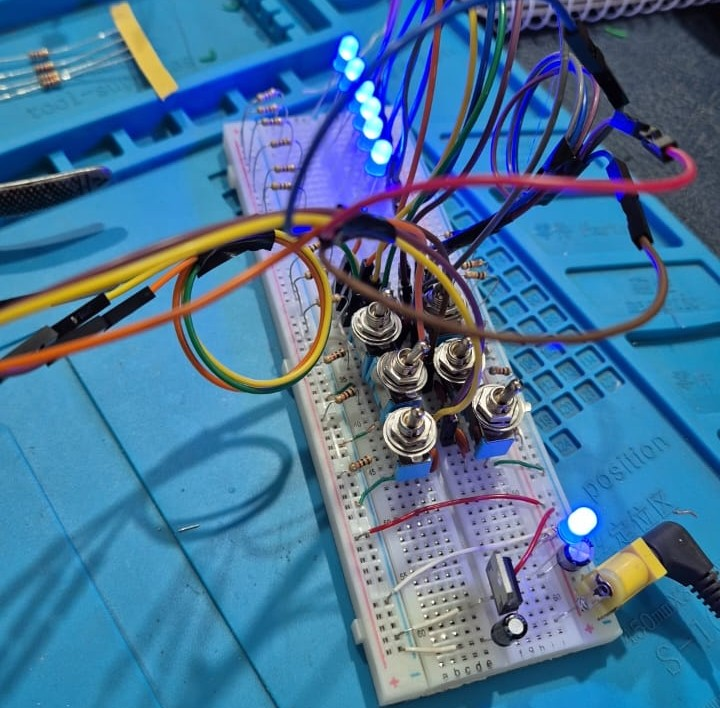
\includegraphics[width=6cm]{./imagenes/portada.jpg}};
    \node at (17cm, -7cm) {\scalebox{5}{\textbf{U}}};
    \node at (17cm, -9cm) {\scalebox{5}{\textbf{T}}};
    \node at (17cm, -11cm) {\scalebox{5}{\textbf{N}}};
    \node at (17cm, -14cm) {\scalebox{5}{\textbf{F}}};
    \node at (17cm, -16cm) {\scalebox{5}{\textbf{R}}};
    \node at (17cm, -18cm) {\scalebox{5}{\textbf{C}}};
    \node at (7.5cm, -14cm) {\scalebox{3}{\textbf{Trabajo práctico Nº1}}};
    \node at (7.5cm, -23.5cm) {
	\begin{minipage}[c]{12cm}
	    \begin{itemize}
            \raggedright
            \item \fontsize{12}{12}\selectfont \textbf{Autores:} 
                \begin{itemize} \item Gonzalo Ezequiel Filsinger - Leg. 403797 \item Ignacio Ismael Perea - Leg. 406265 \item Manuel Leon Parfait - Leg. 406599\end{itemize}
            \item \fontsize{12}{12}\selectfont \textbf{Curso:} 3R1  \\
            \item \fontsize{12}{12}\selectfont \textbf{Asignatura:} Tecnicas Digitales.
            \item \fontsize{12}{12}\selectfont \textbf{Institución:} Universidad Tecnológica Nacional - Facultad Regional de Córdoba.
        \end{itemize}
    \end{minipage}};
\end{tikzpicture}
\restoregeometry
    \renewcommand{\headrulewidth}{0.4pt}
\renewcommand{\footrulewidth}{0.4pt}
\definecolor{textoGris}{HTML}{222222}

\fancypagestyle{fancy}{
    \fancyhf{}

    \fancyfoot[R]{[Filsinger G. - Perea I. - Parfait M.] [\textbf{pág.\ \thepage} de \pageref{LastPage}]}

    \fancyfoot[C]{
        \begin{tikzpicture}[remember picture, overlay]
            \draw[gray!30, line width=0.4pt]
                (0cm, 1cm) -- (0cm, 25cm);
        \end{tikzpicture}
    }

    \fancyhead[L]{
        \begin{tabular}{@{}l@{}}
            \raisebox{-0.5\height}{
\includegraphics[height=0.60in]{./imagenes/logoDepartamentoElectronica.png}}
            \begin{tabular}{@{}l@{}}
                {\color{textoGris}\textbf{Departamento de Ingeniería Electrónica}} \\
                {\color{textoGris}Facultad Regional Córdoba}
            \end{tabular}
        \end{tabular}
    }
}
\titleformat{\section}[hang]{\fontsize{10}{12}\bfseries}{\thesection.}{0.5em}{\underline{#1}}
\titleformat{\subsection}[hang]{\fontsize{10}{11}\bfseries}{\thesubsection.}{0.5em}{#1}
\titleformat{\subsubsection}[hang]{\fontsize{10}{10}\itshape}{\thesubsubsection.}{0.5em}{#1}
\widowpenalty=10000
\clubpenalty=10000
\enlargethispage{-1cm}
    \thispagestyle{empty}
\setcounter{page}{0}
\newpage
\text{}
\clearpage
\onecolumn
\thispagestyle{empty}
\tableofcontents
\clearpage
\twocolumn
\newpage
\thispagestyle{empty}
\setcounter{page}{0}
\text{}
\newpage
    \pagestyle{fancy}

    \section{Actividad 2.1: Conversor de BCD a Exceso-3}

Diseñar y armar un conversor de código BCD a XS3 (exceso 3).
Realizar:
\begin{itemize}
    \item Tabla de verdad.
    \item Obtener las funciones lógicas de salidas con circuitos combinacionales.
    \item Minimizar las funciones canónicas obtenidas de la tabla de verdad.
    \item Armar el circuito y verificar su funcionamiento en el MiniLab.
    \item Armar el circuito y verificar su funcionamiento en el simulador “falstad.com”
\end{itemize}


\subsection{Tabla de verdad}

\begin{center}
\centering
\begin{tabular}{c c c c || c c c c}
A & B & C & D & W & X & Y & Z \\
\hline
0 & 0 & 0 & 0 & 0 & 0 & 1 & 1 \\
0 & 0 & 0 & 1 & 0 & 1 & 0 & 0 \\
0 & 0 & 1 & 0 & 0 & 1 & 0 & 1 \\
0 & 0 & 1 & 1 & 0 & 1 & 1 & 0 \\
0 & 1 & 0 & 0 & 0 & 1 & 1 & 1 \\
0 & 1 & 0 & 1 & 1 & 0 & 0 & 0 \\
0 & 1 & 1 & 0 & 1 & 0 & 0 & 1 \\
0 & 1 & 1 & 1 & 1 & 0 & 1 & 0 \\
1 & 0 & 0 & 0 & 1 & 0 & 1 & 1 \\
1 & 0 & 0 & 1 & 1 & 1 & 0 & 0 \\
1 & 0 & 1 & 0 & x & x & x & x \\
1 & 0 & 1 & 1 & x & x & x & x \\
1 & 1 & 0 & 0 & x & x & x & x \\
1 & 1 & 0 & 1 & x & x & x & x \\
1 & 1 & 1 & 0 & x & x & x & x \\
1 & 1 & 1 & 1 & x & x & x & x \\
\end{tabular}
\\Tabla de verdad para el conversor BCD a Exceso-3
\end{center}

\subsection{Funciones lógicas de salida}
\begin{itemize}
    \item $W = \overline{A} \cdot B \cdot \overline{C} \cdot D + \overline{A} \cdot B \cdot C \cdot \overline{D} + \overline{A} \cdot B \cdot C \cdot D + A \cdot \overline{B} \cdot \overline{C} \cdot \overline{D} + A \cdot \overline{B} \cdot \overline{C} \cdot D$
    \item $X = \overline{A} \cdot \overline{B} \cdot \overline{C} \cdot D + \overline{A} \cdot \overline{B} \cdot C \cdot \overline{D} + \overline{A} \cdot \overline{B} \cdot C \cdot D  + \overline{A} \cdot B \cdot \overline{C} \cdot \overline{D} + A \cdot \overline{B} \cdot \overline{C} \cdot D$
    \item $Y = \overline{A} \cdot \overline{B} \cdot \overline{C} \cdot \overline{D} + \overline{A} \cdot \overline{B} \cdot C \cdot D + \overline{A} \cdot B \cdot \overline{C} \cdot \overline{D} + \overline{A} \cdot B \cdot C \cdot D + A \cdot \overline{B} \cdot \overline{C} \cdot \overline{D}$
    \item $Z = \overline{A} \cdot \overline{B} \cdot \overline{C} \cdot \overline{D} + \overline{A} \cdot \overline{B} \cdot C \cdot \overline{D} + \overline{A} \cdot B \cdot \overline{C} \cdot \overline{D} + \overline{A} \cdot B \cdot C \cdot \overline{D} + A \cdot \overline{B} \cdot \overline{C} \cdot \overline{D}$
\end{itemize}

\saltoPag

\subsection{Minimización por mapas de Karnaugh}



\begin{center}
\centering
\renewcommand{\arraystretch}{1.5}
\begin{tabular}{c|cccc}
\diagbox{AB}{CD} & 00 & 01 & 11 & 10 \\
\hline
00 & 0 & 0 & 0 & 0 \\
01 & 0 & 
    % 0101: grupo 2 (azul)
    \cellcolor{cyan!30}1 & 
    % 0111: grupo 2 (azul) y grupo 3 (verde)
    \tikz{
        \fill[cyan!30] (0,0) rectangle (0.5,0.5);
        \fill[green!30] (0.25,0) rectangle (0.5,0.5);
        \node at (0.25,0.25) {1};
    } & 
    % 0110: grupo 3 (verde)
    \cellcolor{green!30}1 \\
11 & 
    % 1100: grupo 1 (amarillo)
    \cellcolor{red!30}x & 
    % 1101: grupo 1 (amarillo) y grupo 2 (cyan)
    \tikz{
        \fill[red!30] (0,0) rectangle (0.5,0.5);
        \fill[cyan!30] (0.25,0) rectangle (0.5,0.5);
        \node at (0.25,0.25) {x};
    } & 
    % 1111: grupo 1 (amarillo), grupo 2 (cyan), grupo 3 (verde)
    \tikz{
        \fill[red!30] (0,0) rectangle (0.5,0.5);
        \fill[cyan!30] (0.15,0) rectangle (0.35,0.5);
        \fill[green!30] (0.25,0) rectangle (0.5,0.5);
        \node at (0.25,0.25) {x};
    } & 
    % 1110: grupo 1 (amarillo), grupo 3 (verde)
    \tikz{
        \fill[red!30] (0,0) rectangle (0.5,0.5);
        \fill[green!30] (0.25,0) rectangle (0.5,0.5);
        \node at (0.25,0.25) {x};
    } \\
10 & 
    % 1000: grupo 1 (amarillo)
    \cellcolor{red!30}1 & 
    % 1001: grupo 1 (amarillo)
    \cellcolor{red!30}1 & 
    % 1011: grupo 1 (amarillo)
    \cellcolor{red!30}x & 
    % 1010: grupo 1 (amarillo)
    \cellcolor{red!30}x \\
\end{tabular}
Salida W
\end{center}
\begin{itemize}
    \item $W = B\cdot D + B \cdot C + A$
\end{itemize}

\begin{center}
\centering
\renewcommand{\arraystretch}{1.5}
\begin{tabular}{c|cccc}
\diagbox{AB}{CD} & 00 & 01 & 11 & 10 \\
\hline
00 & 0 & 
    % 0001: grupo de 4 (azul)
    \cellcolor{cyan!30}1 & 
    % 0011: grupo de 4 (azul) y grupo de 4 (verde)
    \tikz{
        \fill[cyan!30] (0,0) rectangle (0.5,0.5);
        \fill[green!30] (0.25,0) rectangle (0.5,0.5);
        \node at (0.25,0.25) {1};
    } & 
    % 0010: grupo de 4 (verde)
    \cellcolor{green!30}1 \\
01 & 
    % 0100: grupo de 2 (amarillo)
    \cellcolor{red!30}1 & 0 & 0 & 0 \\
11 & 
    % 1100: grupo de 2 (amarillo)
    \cellcolor{red!30}x & x & x & x \\
10 & 0 & 
    % 1001: grupo de 4 (azul)
    \cellcolor{cyan!30}1 & 
    % 1011: grupo de 4 (azul) y grupo de 4 (verde)
    \tikz{
        \fill[cyan!30] (0,0) rectangle (0.5,0.5);
        \fill[green!30] (0.25,0) rectangle (0.5,0.5);
        \node at (0.25,0.25) {x};
    } & 
    % 1010: grupo de 4 (verde)
    \cellcolor{green!30}x \\
\end{tabular}
Salida X
\end{center}
\begin{itemize}
    \item $X = B \cdot \overline{C} \cdot \overline{D} + \overline{B} \cdot D + \overline{B} \cdot C$
\end{itemize}

\begin{center}
\centering
\renewcommand{\arraystretch}{1.5}
\begin{tabular}{c|cccc}
\diagbox{AB}{CD} & 00 & 01 & 11 & 10 \\
\hline
00 & \cellcolor{cyan!30}1 & 0 & \cellcolor{red!30}1 & 0 \\
01 & \cellcolor{cyan!30}1 & 0 & \cellcolor{red!30}1 & 0 \\
11 & \cellcolor{cyan!30}x & x & \cellcolor{red!30}x & x \\
10 & \cellcolor{cyan!30}1 & 0 & \cellcolor{red!30}x & x \\
\end{tabular}
Salida Y
\end{center}
\begin{itemize}
    \item $Y = \overline{C} \cdot \overline{D} + C \cdot D$
\end{itemize}

\begin{center}
\centering
\renewcommand{\arraystretch}{1.5}
\begin{tabular}{c|cccc}
\diagbox{AB}{CD} & 00 & 01 & 11 & 10 \\
\hline
00 & \cellcolor{red!30}1 & 0 & 0 & \cellcolor{red!30}1 \\
01 & \cellcolor{red!30}1 & 0 & 0 & \cellcolor{red!30}1 \\
11 & \cellcolor{red!30}x & x & x & \cellcolor{red!30}x \\
10 & \cellcolor{red!30}1 & 0 & x & \cellcolor{red!30}x \\
\end{tabular}
Salida Z
\end{center}
\begin{itemize}
    \item $W = \overline{D} $
\end{itemize}

\saltoPag

\subsection{Circuito lógico en Falstad}

\begin{figure}[h!]
    \centering
    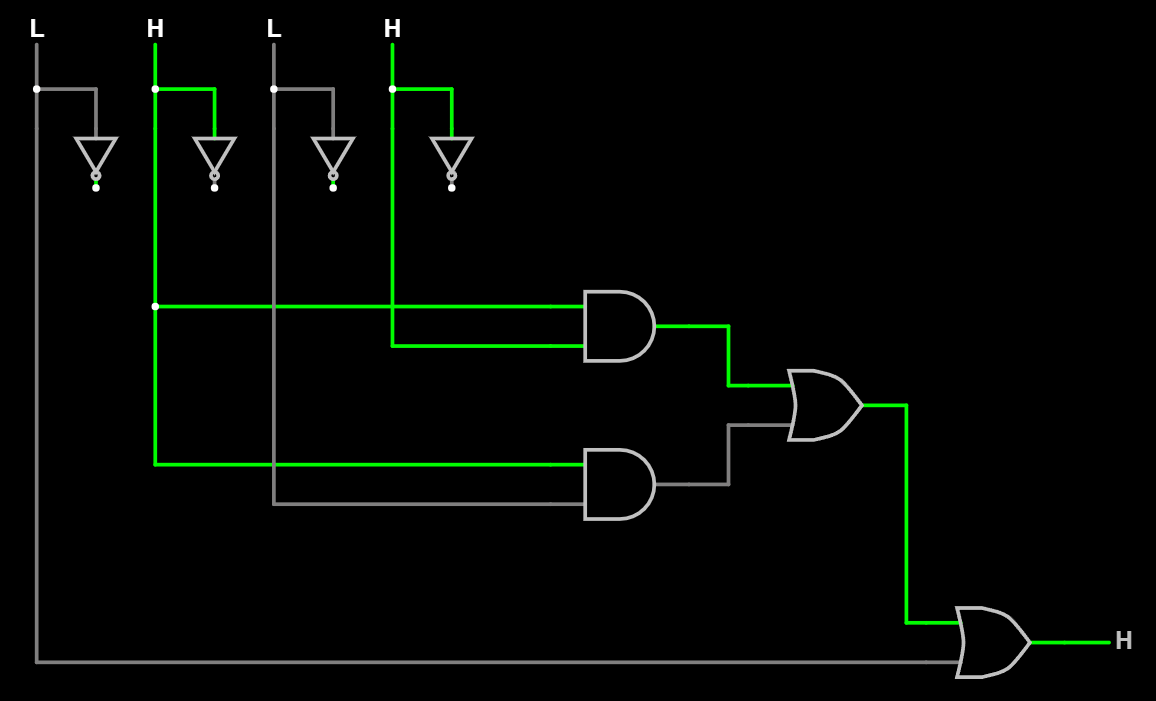
\includegraphics[width=7cm]{imagenes/2.1_W.png}
    \caption{Circuito lógico implementado en Falstad para $W$}
    \footnotesize\textit{Bits usados para ejemplo 0101.}
\end{figure}

\begin{figure}[h!]
    \centering
    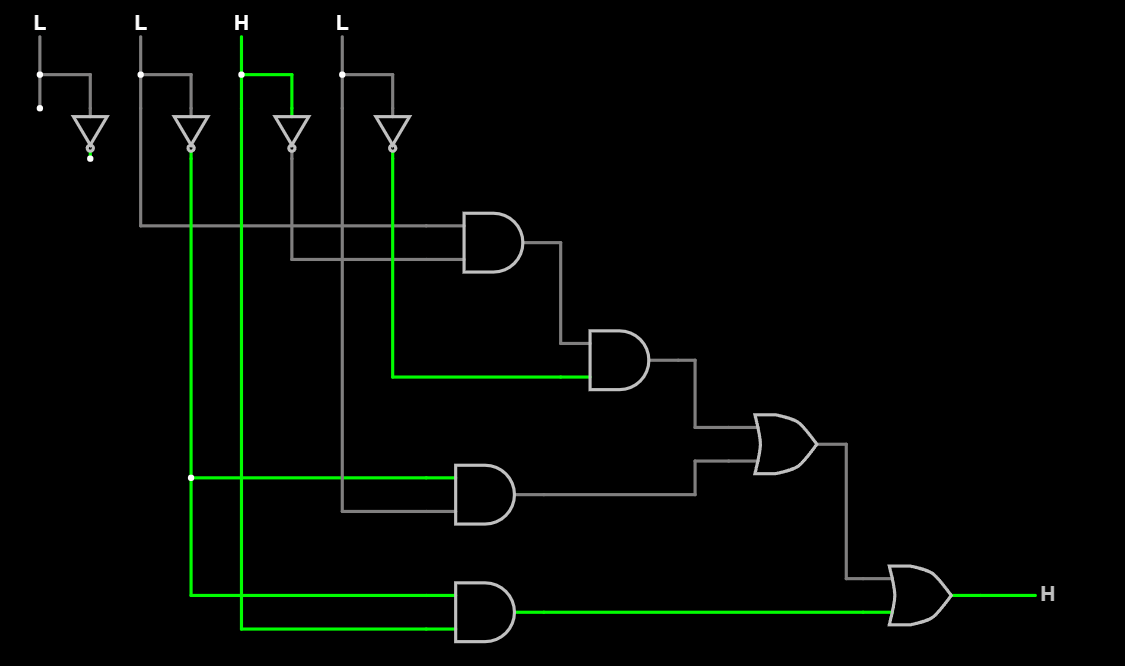
\includegraphics[width=7cm]{imagenes/2.1_X.png}
    \caption{Circuito lógico implementado en Falstad para $X$}
    \footnotesize\textit{Bits usados para ejemplo 0010.}
\end{figure}

\begin{figure}[h!]
    \centering
    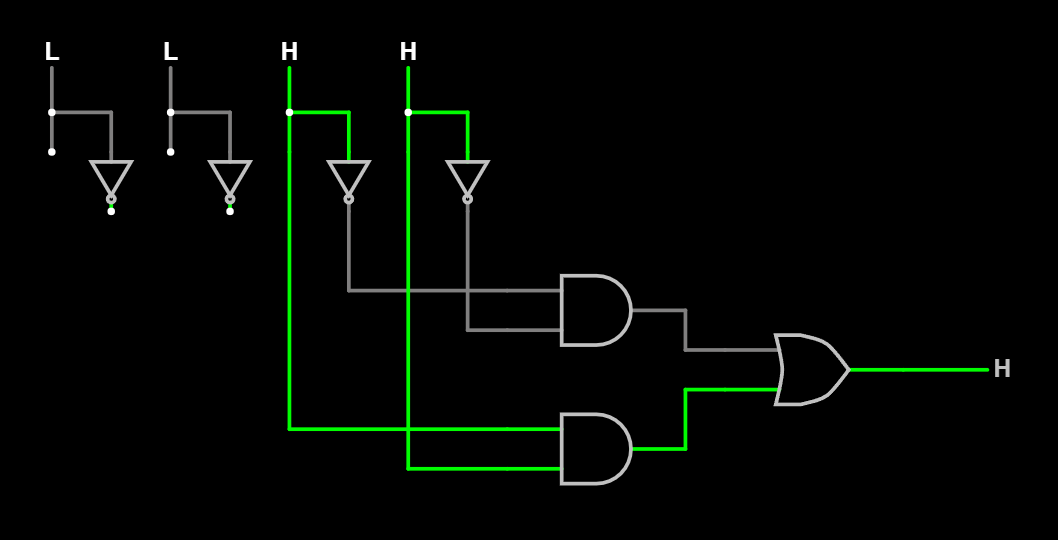
\includegraphics[width=7cm]{imagenes/2.1_Y.png}
    \caption{Circuito lógico implementado en Falstad para $Y$}
    \footnotesize\textit{Bits usados para ejemplo 0011.}
\end{figure}

\begin{figure}[h!]
    \centering
    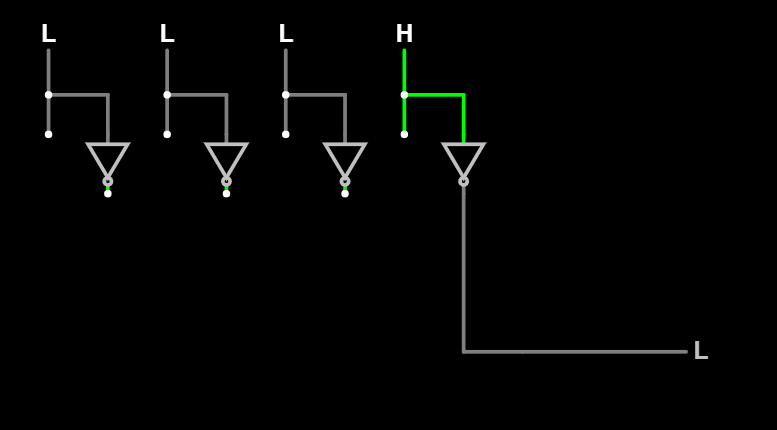
\includegraphics[width=7cm]{imagenes/2.1_Z.png}
    \caption{Circuito lógico implementado en Falstad para $Z$}
    \footnotesize\textit{Bits usados para ejemplo 0001.}
\end{figure}



\saltoPag

\section{Actividad 2.2: Comparador Binario}

El circuito de la figura es un comparador binario de dos números (A y B) de dos bits cada uno. Las
salidas ($S_0$, $S_1$ y $S_2$) representan la salida del comparador y $S0=1$ cuando $A>B$, $S_1= 1$ cuando $A < B$ y
$S_2=1$ $A=B$, en caso de no darse la condición la salida permanece en cero.

% Puedes poner esto en tu archivo actividades.tex donde lo necesites
\begin{figure}[h!]
    \centering
    \begin{tikzpicture}[scale=1, every node/.style={scale=1}]
        % Caja del comparador
        \draw (0,0) rectangle (4,4);
        \node at (2,3.5) {Comparador};

        % Entradas A
        \draw[-] (-1,3) -- (0,3);
        \node[above] at (-0.5,3) {A0};
        \draw[-] (-1,2.5) -- (0,2.5);
        \node[above] at (-0.5,2.5) {A1};
        \node[left] at (-1.3,2.75) {Número A};

        % Entradas B
        \draw[-] (-1,1.5) -- (0,1.5);
        \node[above] at (-0.5,1.5) {B0};
        \draw[-] (-1,1) -- (0,1);
        \node[above] at (-0.5,1) {B1};
        \node[left] at (-1.3,1.25) {Número B};

        % Salidas
        \draw[-] (4,3) -- (5,3);
        \node[above] at (4.5,3) {S0};
        \draw[-] (4,2) -- (5,2);
        \node[above] at (4.5,2) {S1};
        \draw[-] (4,1) -- (5,1);
        \node[above] at (4.5,1) {S2};
    \end{tikzpicture}
    \caption{Comparador binario de dos bits}
\end{figure}

Realizar:
\begin{itemize}
 \item Tabla de verdad.
 \item Obtener las funciones lógicas de salidas con circuitos combinacionales.
 \item Minimizar utilizando mapas de Karnaugh.
 \item Minimizar utilizando los teoremas y postulados del algebra de Boole.
 \item Armar el circuito y verificar su funcionamiento en el MiniLab.
 \item Armar el circuito y verificar su funcionamiento en el simulador “falstad.com”
\end{itemize}



\subsection{Tabla de verdad}

\begin{center}
\centering
\begin{tabular}{c c c c || c c c}
A1 & A0 & B1 & B0 & S0 & S1 & S2 \\
\hline
0 & 0 & 0 & 0 & 0 & 0 & 1 \\
0 & 0 & 0 & 1 & 0 & 1 & 0 \\
0 & 0 & 1 & 0 & 0 & 1 & 0 \\
0 & 0 & 1 & 1 & 0 & 1 & 0 \\
0 & 1 & 0 & 0 & 1 & 0 & 0 \\
0 & 1 & 0 & 1 & 0 & 0 & 1 \\
0 & 1 & 1 & 0 & 0 & 1 & 0 \\
0 & 1 & 1 & 1 & 0 & 1 & 0 \\
1 & 0 & 0 & 0 & 1 & 0 & 0 \\
1 & 0 & 0 & 1 & 1 & 0 & 0 \\
1 & 0 & 1 & 0 & 0 & 0 & 1 \\
1 & 0 & 1 & 1 & 0 & 1 & 0 \\
1 & 1 & 0 & 0 & 1 & 0 & 0 \\
1 & 1 & 0 & 1 & 1 & 0 & 0 \\
1 & 1 & 1 & 0 & 1 & 0 & 0 \\
1 & 1 & 1 & 1 & 0 & 0 & 1 \\
\end{tabular}
\\Tabla de verdad del comparador binario de dos bits
\end{center}


\subsection{Funciones lógicas de salida}
\begin{itemize}
    \item $S0 = \overline{A_1} \cdot A_0 \cdot \overline{B_1} \cdot \overline{B_0} + A_1 \cdot \overline{A_0} \cdot \overline{B_1} \cdot \overline{B_1} + A_1 \cdot \overline{A_0} \cdot \overline{B_1} \cdot B_0 + A_1 \cdot A_0 \cdot \overline{B_1} \cdot \overline{B_0} + A_1 \cdot A_0 \cdot \overline{B_1} \cdot B_0 + A_1 \cdot A_0 \cdot B_1 \cdot \overline{B_0}$
    \item $S1 = \overline{A_1} \cdot \overline{A_0} \cdot \overline{B_1} \cdot B_0 + \overline{A_1} \cdot \overline{A_0} \cdot B_1 \cdot \overline{B_0} + \overline{A_1} \cdot \overline{A_0} \cdot B_1 \cdot B_0 + \overline{A_1} \cdot A_0 \cdot B_1 \overline{B_0} + \overline{A_1} \cdot A_0 \cdot B_1 \cdot B_0 + A_1 \cdot \overline{A_0} \cdot B_1 \cdot B_0 $ 
    \item $S2 = \overline{A_1} \cdot \overline{A_0} \cdot \overline{B_1} \cdot \overline{B_0} + \overline{A_1} \cdot A_0 \cdot \overline{B_1} \cdot B_0 + A_1 \cdot \overline{A_0} \cdot B_1 \cdot \overline{B_0} + A_1 \cdot A_0 \cdot B_1 \cdot B_0 $
\end{itemize}


\subsection{Minimización por mapas de Karnaugh}

\begin{center}
\centering
\renewcommand{\arraystretch}{1.5}
\begin{tabular}{c|cccc}
\diagbox{$A_1A_0$}{$B_1B_0$} & 00 & 01 & 11 & 10 \\
\hline
00 & 0 & 0 & 0 & 0 \\
01 & \cellcolor{cyan!30}1 & 0 & 0 & 0 \\
11 & 
    % 1100: tres colores, cada uno ocupa un tercio vertical de la celda
    \tikz{
        \fill[red!30] (0,0) rectangle (0.2,0.5);
        \fill[cyan!30] (0.2,0) rectangle (0.4,0.5);
        \fill[green!30] (0.4,0) rectangle (0.6,0.5);
        \node at (0.3,0.3) {1};
    } &
    \cellcolor{red!30}1 & 0 & \cellcolor{green!30}1 \\
10 & 
    \cellcolor{red!30}1 & 
    \cellcolor{red!30}1 & 
    0 & 
    0 \\
\end{tabular}
\\Mapa de Karnaugh para $S_0$ con la celda 1100 mostrando los tres colores
\end{center}

\begin{itemize}
    \item \textbf{Grupo rojo:} 1100, 1101, 1000, 1001.
    \item \textbf{Grupo cyan:} 0100 y 1100.
    \item \textbf{Grupo verde:} 1110 y 1100.
\end{itemize}

\begin{itemize}
    \item $S_0 = A_1 \cdot \overline{B_1} + A_0 \cdot \overline{B_1} \cdot \overline{B_0} + A_1 \cdot A_0 \cdot \overline{B_0}$
\end{itemize}

\begin{center}
\centering
\renewcommand{\arraystretch}{1.5}
\begin{tabular}{c|cccc}
\diagbox{$A_1A_0$}{$B_1B_0$} & 00 & 01 & 11 & 10 \\
\hline
00 & 0 & 
    % 0001: grupo 2 (cyan)
    \cellcolor{cyan!30}1 & 
    % 0011: grupo 1 (rojo), grupo 2 (cyan), grupo 3 (verde)
    \tikz{
        \fill[red!30] (0,0) rectangle (0.2,0.5);
        \fill[cyan!30] (0.2,0) rectangle (0.4,0.5);
        \fill[green!30] (0.4,0) rectangle (0.6,0.5);
        \node at (0.3,0.3) {1};
    } & 
    % 0010: grupo 1 (rojo)
    \cellcolor{red!30}1 \\
01 & 0 & 0 & 
    % 0111: grupo 1 (rojo)
    \cellcolor{red!30}1 & 
    % 0110: grupo 1 (rojo)
    \cellcolor{red!30}1 \\
11 & 0 & 0 & 0 & 0 \\
10 & 0 & 0 & 
    % 1011: grupo 3 (verde)
    \cellcolor{green!30}1 & 0 \\
\end{tabular}
\\Mapa de Karnaugh para $S_1$ con agrupaciones
\end{center}


\begin{itemize}
    \item \textbf{Grupo rojo:} 0011, 0010, 0111, 0110.
    \item \textbf{Grupo cyan:} 0001 y 0011.
    \item \textbf{Grupo verde:} 1011.
\end{itemize}

\begin{itemize}
    \item $S_1 = \overline{A_1} \cdot B_1 + \overline{A_1} \cdot \overline{A_0} \cdot B_0 + B_1 \cdot B_0 \cdot \overline{A_0}$
\end{itemize}



\begin{center}
\centering
\renewcommand{\arraystretch}{1.5}
\begin{tabular}{c|cccc}
\diagbox{$A_1A_0$}{$B_1B_0$} & 00 & 01 & 11 & 10 \\
\hline
00 & 1 & 0 & 0 & 0 \\
01 & 0 & 1 & 0 & 0 \\
11 & 0 & 0 & 1 & 0 \\
10 & 0 & 0 & 0 & 1 \\
\end{tabular}
\\Mapa de Karnaugh para $S_2$
\end{center}

\begin{itemize}
    \item $S_2 = \overline{A_1} \cdot \overline{A_0} \cdot \overline{B_1} \cdot \overline{B_0} + \overline{A_1} \cdot A_0 \cdot \overline{B_1} \cdot B_0 + A_1 \cdot \overline{A_0} \cdot B_1 \cdot \overline{B_0} + A_1 \cdot A_0 \cdot B_1 \cdot B_0$
\end{itemize}

En este caso, Karnaugh no es util para al simplificar, por lo que debemos hacerlo mediante los teoremas y postulados del álgebra de Boole.

\begin{itemize}
    \item $S_2 = \overline{A_1} \cdot \overline{A_0} \cdot \overline{B_1} \cdot \overline{B_0} + \overline{A_1} \cdot A_0 \cdot \overline{B_1} \cdot B_0 + A_1 \cdot \overline{A_0} \cdot B_1 \cdot \overline{B_0} + A_1 \cdot A_0 \cdot B_1 \cdot B_0$
    \item $(\overline{A_1} \cdot \overline{B_1}) \cdot (\overline{A_0} \cdot \overline{B_0} + A_0 \cdot B_0) + (A_1 \cdot B_1) \cdot (A_0 \cdot B_0 + \overline{A_0} \cdot \overline{B_0})$
    \item $ \overline{A_1} \cdot \overline{B_1} \cdot (\overline{A_0 \oplus B_0}) + A_1 \cdot B_1 \cdot (\overline{A_0 \oplus B_0})$
    \item $(\overline{A_0 \oplus B_0}) \cdot (\overline{A_1 \oplus B_1})$
\end{itemize}

\subsection{Circuito lógico en Falstad}

\begin{figure}[h!]
    \centering
    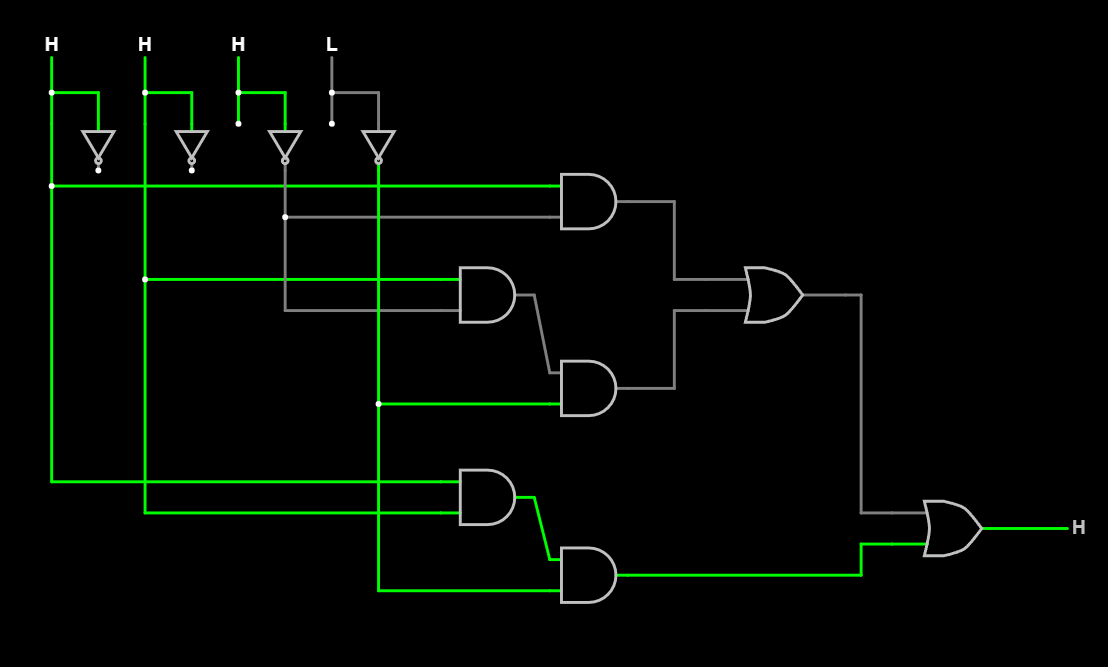
\includegraphics[width=7cm]{imagenes/2.2_S0.png}
    \caption{Circuito lógico implementado en Falstad para $S_2$}
    \footnotesize\textit{Bits usados para ejemplo 1110.}
\end{figure}


\begin{figure}[h!]
    \centering
    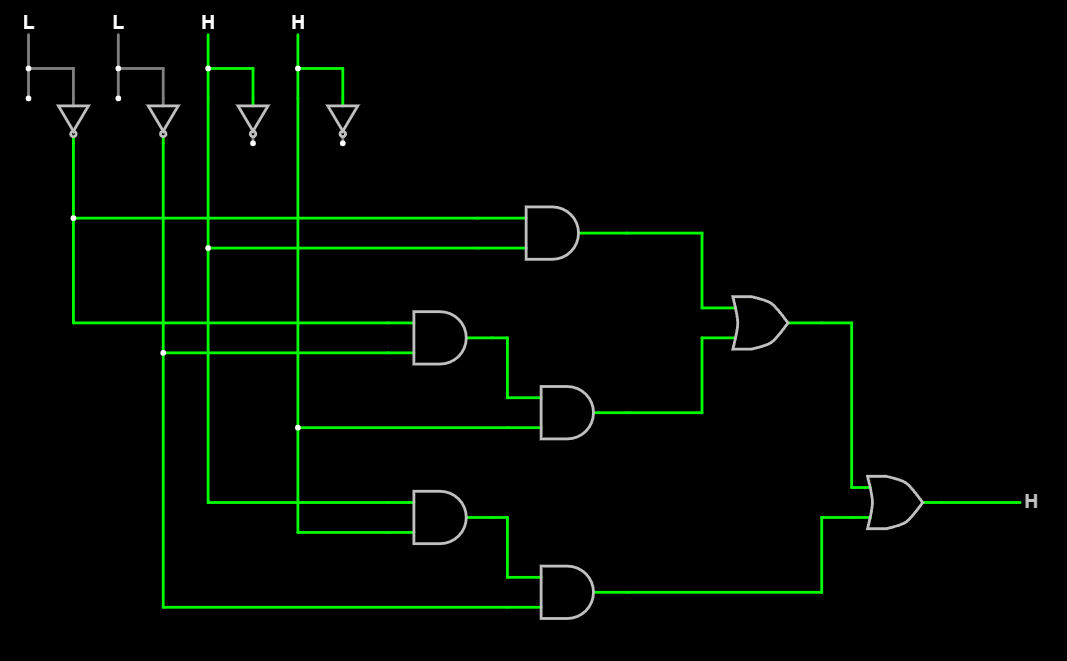
\includegraphics[width=7cm]{imagenes/2.2_S1.png}
    \caption{Circuito lógico implementado en Falstad para $S_2$}
    \footnotesize\textit{Bits usados para ejemplo 0011.}
\end{figure}


\begin{figure}[h!]
    \centering
    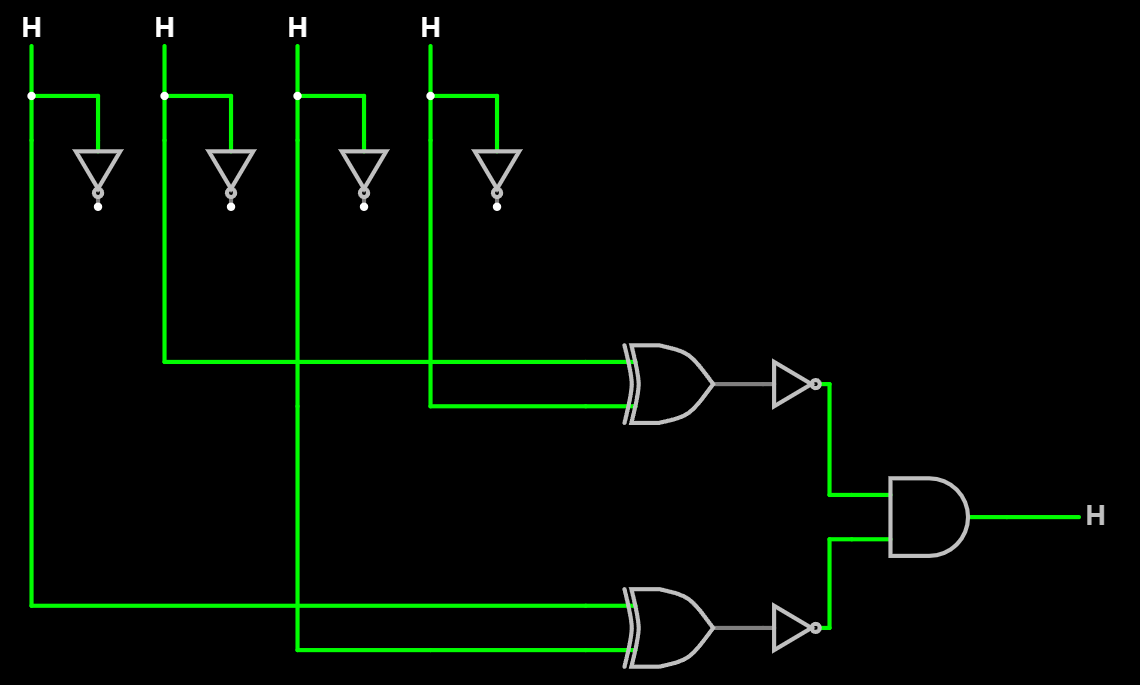
\includegraphics[width=7cm]{imagenes/2.2_S2.png}
    \caption{Circuito lógico implementado en Falstad para $S_2$}
    \footnotesize\textit{Bits usados para ejemplo 1111.}
\end{figure}


\section{Imagenes de Circuitos}


\subsection{Circuito 2.1}

    Materiales utilizados:
    \begin{itemize}
        \item 1 CD4069 (Inversor)
        \item 2 CD4081 (AND)
        \item 2 CD4071 (OR)
        
    \end{itemize}

    Circuito lógico implementado en protoboard para la actividad 2.1
    \begin{center}
    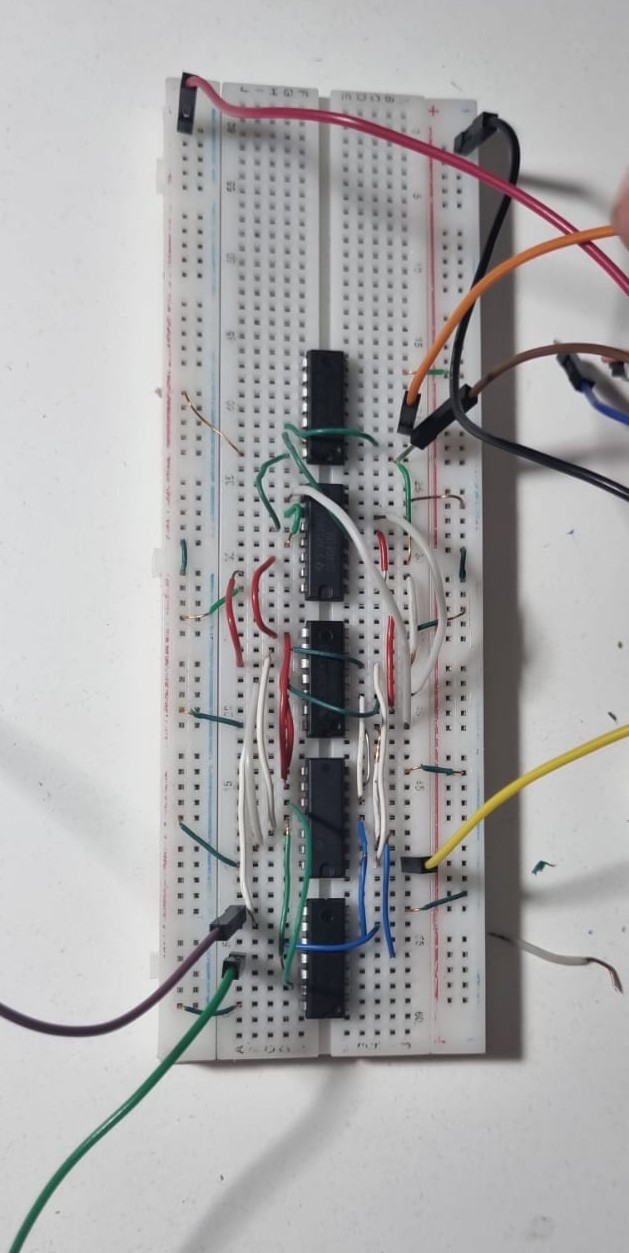
\includegraphics[width=6.3cm]{imagenes/Circuito1.jpg}
    \end{center}

\saltoPag

\subsection{Circuito 2.2}

    Materiales utilizados:
    \begin{itemize}
        \item 1 CD4069 (Inversor)
        \item 3 CD4081 (AND)
        \item 1 CD4071 (OR)
        \item 1 CD4077 (XOR)
    \end{itemize}
Circuito lógico implementado en protoboard para la actividad 2.2
    \begin{center}
        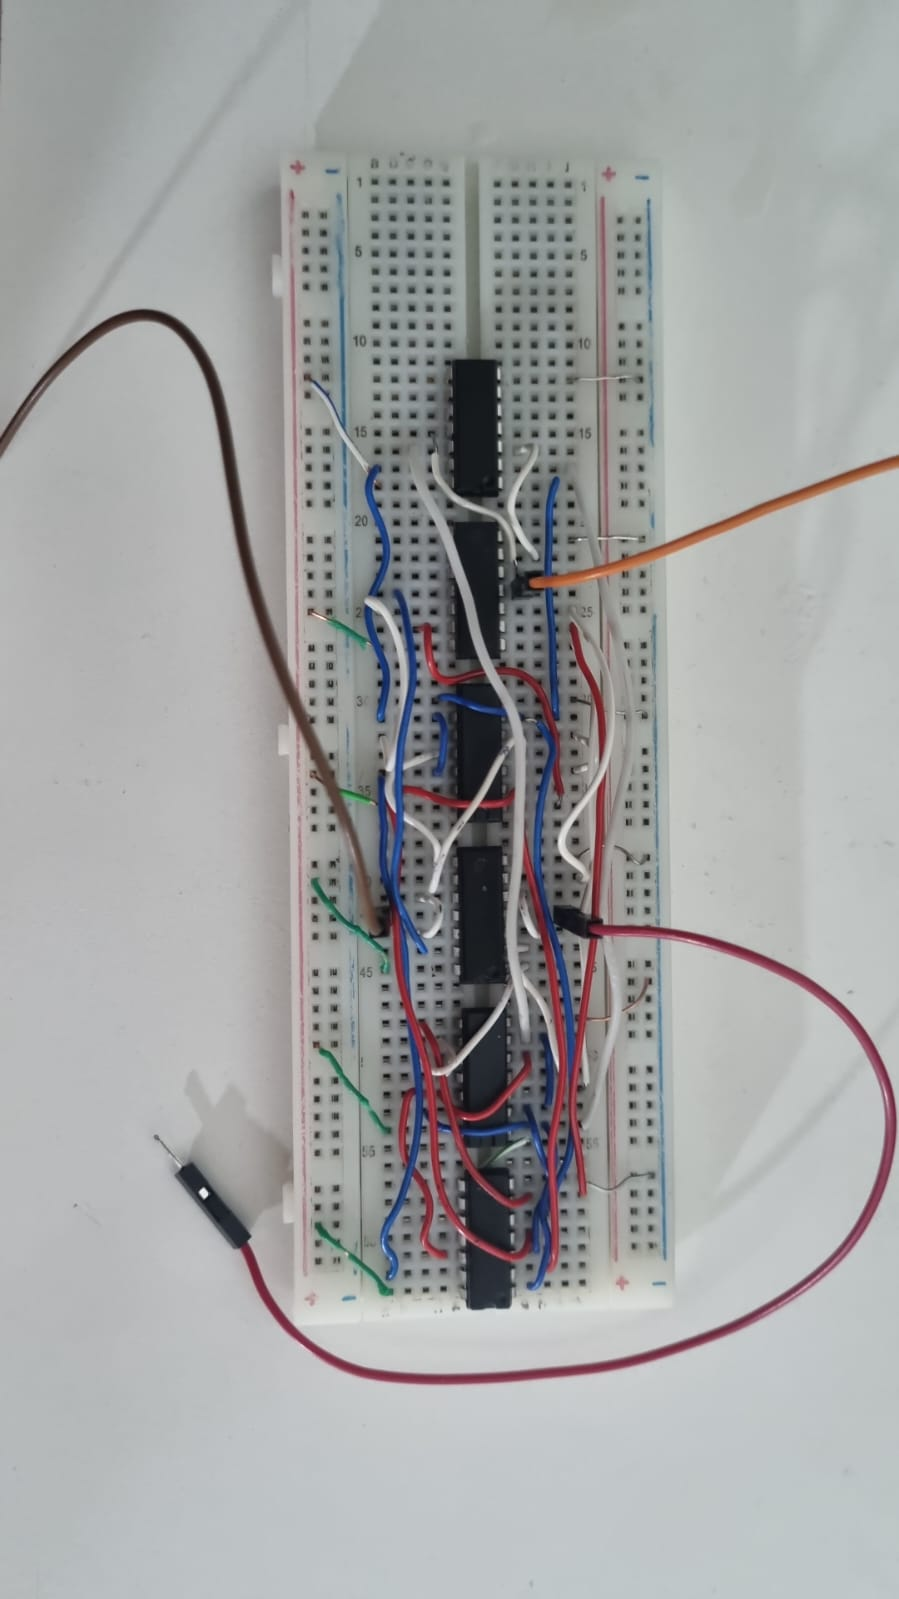
\includegraphics[width=7cm]{imagenes/Circuito2.jpg}
        \end{center}

        \section{Conclusiones}

        Como conclusión a estas actividades podemos decir que el método de minimización por mapa de Karnaugh algunas veces se puede complementar con el álgebra de Boole, ya que en alguno de los casos luego de realizar el mapa fue posible seguir simplificando la expresión obtenida, también en este trabajo se hizo uso de los términos "don't care". Además se pudo lograr con éxito la implementación tanto mediante simulación como física con el uso del MiniLab.
    


\end{document}